\chapter{Theoretical introduction}
\label{ch:theory}

\section{Thermoelectricity in the quantum realm}
\label{sec:teo:teoThermoQH}

A central concept we will exploit is the use of a \textit{transmission function} $\mathcal{T}$ as means to model different aspects of our coherent systems. Since we are dealing with non-equilibrium thermodynamics we will be using known results of linear response theory and Onsager reciprocity relations \cite{onsager1931reciprocalI,onsager1931reciprocalII}, extended later by Mazur and de Groot \cite{mazur1953onsager} to systems under external magnetic fields. 
We will follow many times a beatifull and extended review by Benenti, Casati, Saito and Whitney \cite{benenti2017fundamental} on this subject matter, in many cases we will not go deep into the theory, in those cases this review already covers perfectly the necessary theory. A second review of main importance is the one by Giazotto, et. al. \cite{Giazotto2006Mar}, where the theoretical approach is deeply embedded of experimental examples, and is also an important source of information on the subject.

One could argue about the time-reversal symmetry and its consecuences, but it has been taken into consideration recently \cite{luo2020onsager}.

A key argument is that we will be dealing always with low dimensional systems that can be modeled as two terminal systems, having chiral (directional) coherent channels connecting these terminals, as shown in figure. 

As we have briefly mentioned, topologycal insulators (as the quantum Hall state) provide such particular configurations. Lets discuss then the basic mathematical approach that we will use latter.

\begin{figure}
    \centering
    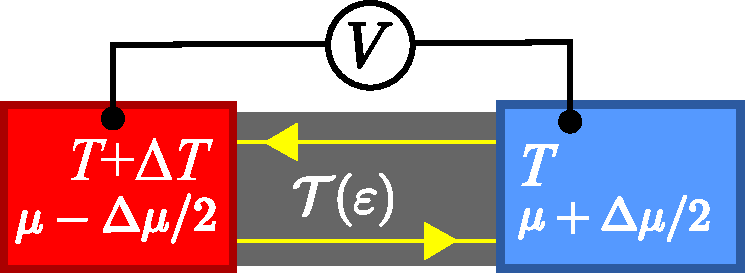
\includegraphics[width = 0.5\textwidth]{figures/theory/2-terminal.pdf}
    \caption{Schematic view of a typical topological system having two coherent chirial edge channels. It is also included a possible difference in temperature and chemical potential between contacts. Such systems can be completely described by a transmission function $\trans(\varepsilon)$. A configuration like this will produce a voltage accordingly, here indicated to be measured by the ideal voltmeter $V$.}
    \label{fig:teo:2terminal}
\end{figure}


In linear response, the corresponding charge and heat currents for small  $\Delta T$ and bias voltage $V$
 can be expressed as \cite{benenti2017fundamental}
 %
\begin{equation}
\label{eq:thermoLinearMatrix}
    \left(
        \begin{array}{c}
            I^C/e \\
            I^Q 
        \end{array}
    \right)  
    =  
    \left(
        \begin{array}{cc}
            \onsa{11}   &   \onsa{12}  \\
            \onsa{21}   &   \onsa{22} 
        \end{array}
    \right) 
    \left(
        \begin{array}{c}
            e \text{V} / k T\\
            \Delta T / k T^2
        \end{array}
    \right),
\end{equation}
%
$\hat{\cal L}$ is the Onsager matrix \cite{onsager1931reciprocalI, onsager1931reciprocalII} wile the right vector contains the so called . 

This leads to the definition of the usual thermoelectric variables:
\begin{itemize}
  \item The electrical conductance $G=e^2 \onsa{11}/T$
  \item The thermal conductance $\kappa= \det{\hat{\cal L}}/\left(T^2 \onsa{11} \right)$
  \item The Seebeck coefficient $S  = \onsa{12}/ \onsa{11}$
  \item The Peltier coefficient $\Pi= \onsa{21}/ \onsa{11}$
\end{itemize}

For ballistic or diffusive transport  ${\cal L}_{ij}$ depends only on the quantum dynamics of the electrons in the presence of the magnetic field and the disorder of the sample. They are  described by a transmission function $\trans (\varepsilon)$,
%
\begin{equation}
  \label{eq:teo:onsaCoef}
  \onsa{ij}= - T \int  \frac{\partial f (\varepsilon)}{\partial \varepsilon} \left(\varepsilon-\mu \right)^{i+j-2} {\cal T}(\varepsilon) \frac{d\varepsilon}{h},
\end{equation}
%
where  $f(\varepsilon)=1/(e^{(\varepsilon-\mu)/k T}+1)$ is the Fermi-Dirac distribution function, $\mu$ is the chemical potential and $T$ is the temperature of the carriers. 

We will apply this formalism to a specific initial problem in the next section, it will allow us to understand its consequences and possibilities. As we have discussed such studies in quantum coherent systems are of great significance in order to control heat to work conversion, heat distribution, carrier heat transport, heat filtering, thermovoltage, peltier effect, between many others \textcolor{red}{citar papers de control térmico de electrones en estados coherentes en cada uno de los ejemplos dados}.


\section{Onsager formalism applied to a\\ topologycal insulator problem}
\label{sec:teo:onsaTopo}


During the initial course of this thesis, when  learning the Onsager formalism, the idea to study thermoelectricity and heat control also in quantum spin Hall states (QSH) was suggested. Having the possibility to apply both, the tools in need and to explore the new realm of two-dimensional (2D) topological insulators (TIs). This systems are another beatiful realization of quantum coherent transport.\textcolor{red}{agregar citas de choerent transport}

Like the quantum hall state the quantum spin Hall state hosts edge states (channels)\cite{nowack2013imaging}, 
examples being \ce{MnBi2Te4 / Bi2Te3} heteroestructures and \ce{CdTe/HgTe} quantum wells \cite{konig2008quantum, Koenig766,bernevig2006quantum,bernevig2006prl,bernevig2006qsh}. 
Unlike the QHE they do not require magnetic fields to be applied, here the particular band structure of the system produces a sequence of states resulting in the quantum spin Hall (QSH) state. It take place in 2D-TIs, and preserves time-reversal invariance. Hence, helical pairs of edge states appear, these are the \textit{helical Kramers pairs} \cite{kanemele2005,bernevig2006quantum,Koenig766, Roth2009} having opposite spin orientations determined by the spin orbit of the system.

We will not go deeper into these impressive systems, bibliography already covers them, for example \cite{maciejko2011quantum, konig2008quantum}. Also very interesting information can be found at groups webpages, particularly \url{https://www.bernevig.com/} and \url{https://imprs-cpqm.mpg.de/93235/LP_Molenkamp}.

Finally, 2D-TIs will be in the future of metrology, recent works by the Electrical quantum metrology group at PTB (Physikalisch-Technische bundesanstalt) and Molenkamp group at MPI (Max Planck Institute) have demonstrated the universality of the effect applying cutting edge metrology to \ce{V_{0.1}(Bi_{0.21} Sb_{0.79})_{1.9}Te3 } compounds \cite{gotz2018zero}. 


\subsubsection{Thermoelectric performance in the quantum coherent regime}

The initial theoretical (but realistic) problem studied, consisted in the device shown in figure \ref{fig:teo:QSHscheme}, an original idea of Dr. Arrachea that was developed with D. Gresta and myself \cite{Gresta2019}.

\begin{figure}
    \centering
    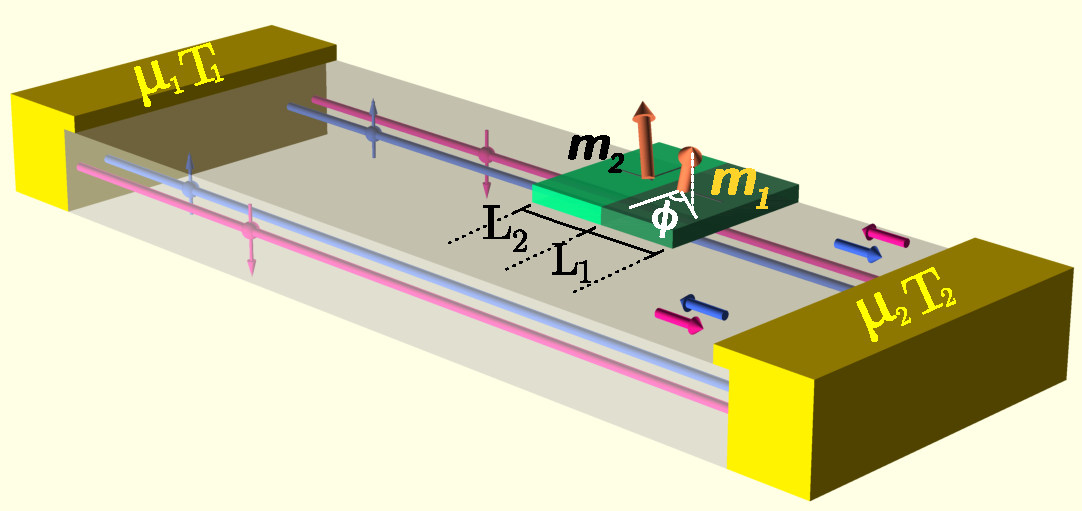
\includegraphics[width = 0.7\textwidth]{figures/theory/QSHscheme.pdf}
    \caption{Sketch of the setup scheme. 2D TI contacted to ohmic contacts at which a bias voltage $e$V$ = \mu_1−\mu_2$ and temperature difference $\Delta T = T_2 - T_1$ are applied. Two nano-magnets having moments $\textbf{m}_1$ and $\textbf{m}_2$ and lengths $L_1$ and $L_2$, are contacted to a helical Kramer's pair of edge states.}
    \label{fig:teo:QSHscheme}
\end{figure}

The system consist on a 2D topological insulator having two ohmic contacts at different temperatures ($T_1, T_2$) and chemical potentials ($\mu_1, \mu_2$), and two nanomagnetic islands over a side of the sample, only affecting one pair of the helical edge states. We shall start by studying a single island and then consider two of them, having different magnetic moments. The relevant physical property will be the the finite component of those moments perpendicular to the direction of the spin-orbit interaction of the 2D-TI, similar systems were considered in Refs. \cite{silvestrov2016noiseless,arrachea2015nanomagnet}. The system can also be studied to produce topological superconductivity \cite{Fu2009}.  

Such system is coherent, so its transport properties do not present inelastic scattering processes, and can be \textit{fully characterized by a transmission function.} Furthermore, the off-diagonal components $\mathcal{L}_{12} = \mathcal{L}_{21}$ are the ones encoding the thermoelectric heat to work conversion. 
As a general rule, when searching for optimal thermoelectric systems, one must search for systems having a rapidly changing transmission function within the relevant transport window. In those energy ranges we will be able to break the particle-hole symmetry, a necessary condition for heat to work conversion. 

This idea is key throughout this thesis, particularly when studying thermoelectricity in the quantum Hall state, in which the mentioned change is obtained on the sides of the mobility gap, see \ref{ch:vtp_g_model}.

The performance of the system is usually measured by the \textit{figure of merit ZT}, being its limit the one of Carnot, then $ZT \rightarrow{\infty}$, obtained for delta-shaped distributions \cite{mahan1996best}. Meanwhile, thermoelectric heat engines (power from heat) is optimized for the case of Heaviside step functions.

Typical temperatures for such devices mean to work at sub-kelvin temperatures to ensure full quantization, even when theoretically some of them should perform up to \SI{100}{\kelvin} \cite{pan2020probing}. Regarding the magnetic islands, let us start by considering a single magnetic domain having a magnetization $\textbf{m}$, which projection to the perpendicular direction to the helical states is $\phi$ and having a length $L$. 

\textcolor{red}{Probably I could skip the Hamiltonian, just state the mag moment and say that: Solving the Dirac hamiltonian plus the magnetic interaction, eq. \ref{eq:teo:magMoment} to the Kramer's pairs \cite{BustosMarun2013,Gresta2019,Gresta2021PhD}, we find the transmission function to be... }
To obtain the  transmission function one must start by modeling the system via the usual Dirac Hamiltonian of the Kramer's pairs plus a magnetic interaction
\begin{equation}
\label{eq:teo:hamiltonianQSH}
    \textit{H} = 
        \int{
        \Psi^\dagger(x)
        \left[ 
            \left( 
                -i\hbar \upsilon_F \partial_x
            \right) 
            \hat{\sigma}_z + J \, \textbf{m}(x) \cdot \hat{\boldsymbol{\sigma}}
        \right]
        \Psi^\dagger(x)
        }
\end{equation}
the Kramer's pairs wavefunctions $\Psi(x) = \left( \psi_{R\uparrow}(x),\psi_{L\downarrow} \right)^T$ include the right (left) moving carrier channels having velocity $\upsilon_F$ and $\uparrow$ (\downarrow) spin orientation. $J$ represents the magnetic exchange interaction between the magnetic moment of the island and the spin of the carriers. Fianlly, $\hat{\textbf{\sigma}} = \left( \hat{\sigma}_x,\hat{\sigma}_y, \hat{\sigma}_z \right)$ are the usual Pauli matrices.

Meanwile, the magnetic moment is given by
\begin{align}
\begin{split}
\label{eq:teo:magMoment}
    \textbf{m}(x) = \sum_{j=1}^N{\Theta(x_j - x)\Theta(x - x_{j-1})\textbf{m}_j}\\
    \textbf{m}_j = (m_{j\perp} \cos{\phi_j}, m_{j\perp} \sin\phi_j, m_{j\parallel}) 
\end{split}
\end{align}
$\textbf{m}_j$ being the magnetic moment per unit length of the islands having lengths $L_j = x_j - x_{j-1}$. Here $\perp$, $\parallel$ means respect to the direction of the spin orbit interaction of the TI. 
We shall start by discussing the $N = 1$ problem and mention some interesting additional effects when $N = 2$.

\subsubsection{Single domain case}
Solving this Hamiltonian problem as in Refs.~\cite{BustosMarun2013,Gresta2019,Gresta2021PhD} results, for the case of a \textit{single magnetic island} $N=1$, in the following transmission function 
\begin{align}
    \label{eq:teo:transFuncQSH}
    \trans(\varepsilon) &= \frac{\mid \varepsilon^2_\perp - \varepsilon^2 \mid}{\mid \varepsilon^2_\perp - \varepsilon^2 \mid \cos^2{\lambda} + \varepsilon^2 \sin^2{\lambda}}\\
    \lambda &= \frac{L}{L_0}\sqrt{\left( \varepsilon/\varepsilon_{\perp} \right)^2-1} = lr 
\end{align}
where $l = L/L_0$, $L_0 = \hbar \upsilon_F/\varepsilon_{\perp}$ and  $r=\sqrt{\left( \varepsilon/\varepsilon_{\perp} \right)^2-1}$. It is important to note two things regarding the transmission function:
\begin{itemize}
    \item Only depends on the perpendicular projection of the moment $m_{\perp}$ to the spin-orbit interaction of the material. 
    \item It is not symmetrical respect to $\varepsilon =0$, this means that there is an effective coupling of the Kramer pairs, resulting in a gap opening in $\varepsilon_{\perp}$.
\end{itemize}

The resulting behiviour of the system is shown in Fig.~\ref{fig:teo:tau1isla}, where the horizontal axis is normalized to $\varepsilon_{\perp}$, as mentioned we find a gap opening for once we 





\begin{figure}
    \centering
    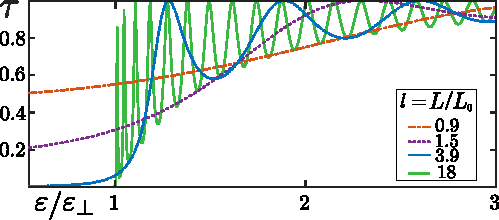
\includegraphics[width = 0.5\textwidth]{figures/theory/fig2.pdf}
    \caption{Tau}
    \label{fig:teo:tau1isla}
\end{figure}

\begin{figure}
    \centering
    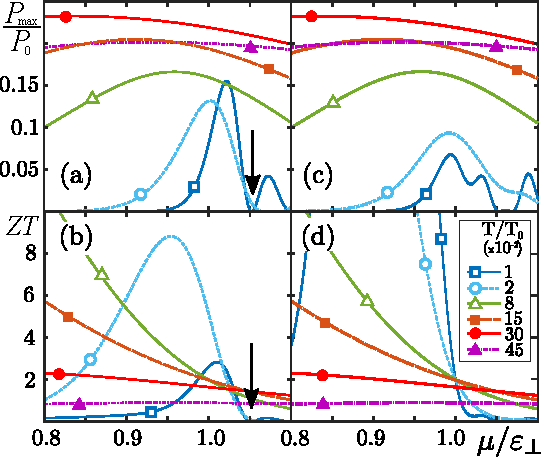
\includegraphics[width = 0.5\textwidth]{figures/theory/fig3.pdf}
    \caption{power and ZT}
    \label{fig:teo:powerZT}
\end{figure}

\begin{figure}
    \centering
    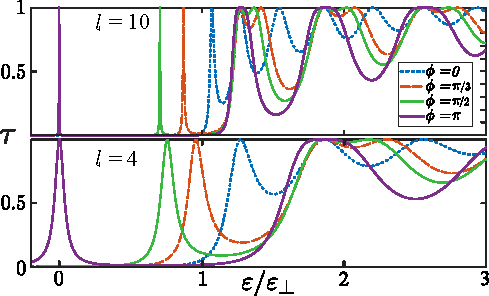
\includegraphics[width = 0.5\textwidth]{figures/theory/fig4.pdf}
    \caption{Tau for two islands and different L}
    \label{fig:teo:tauDiffL}
\end{figure}

\begin{figure}
    \centering
    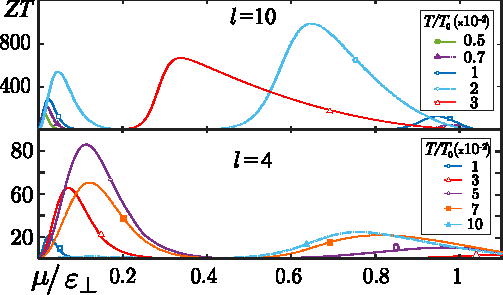
\includegraphics[width = 0.5\textwidth]{figures/theory/fig5.pdf}
    \caption{power and ZT two islands different L}
    \label{fig:teo:powerZTDiffL}
\end{figure}


\begin{figure}
    \centering
    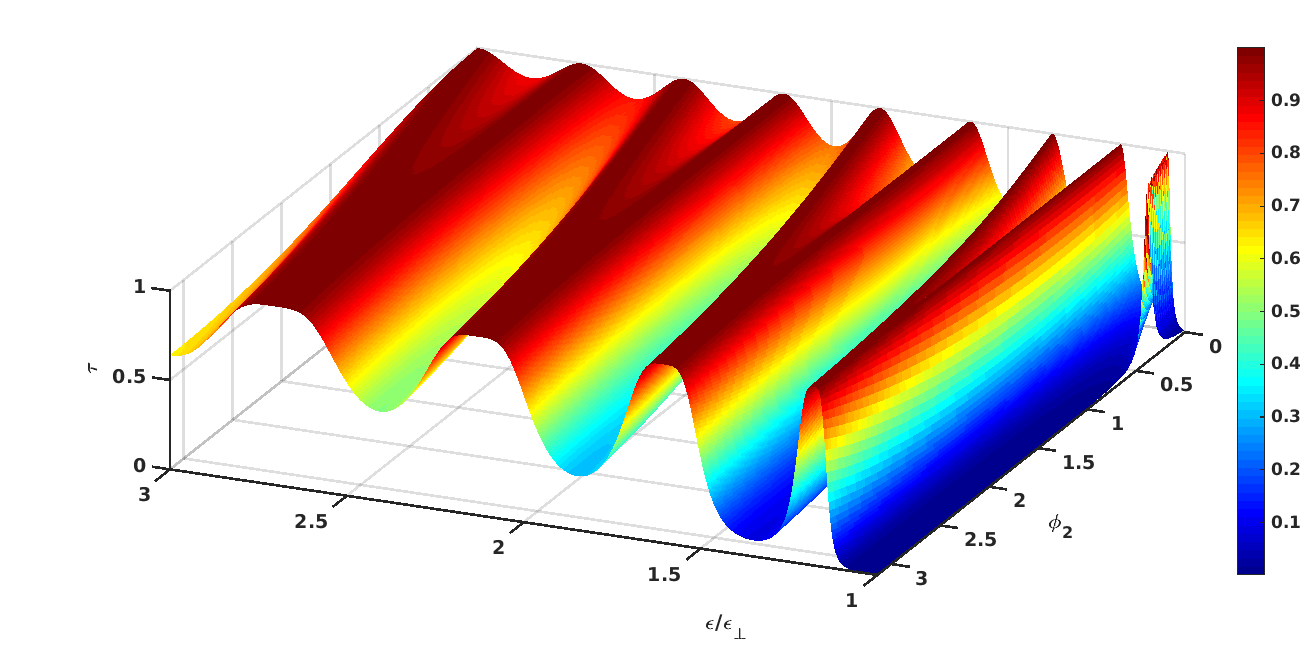
\includegraphics[width = 0.5\textwidth]{figures/theory/Tauenerphi.png}
    \caption{Tau for changing relative angle}
    \label{fig:teo:tauDiffangle}
\end{figure}